\documentclass[12pt, twoside]{book}
\usepackage{lipsum}
%-------------------------------------------------------------------------------------------
%%%%%%%%%%%%%%%%%%%%%%%%%%%%%%% Geometry and font
\usepackage[utf8]{inputenc}
\usepackage{times}
\usepackage[margin=1.0in]{geometry}
%\geometry{bindingoffset=1cm} %% disable this until final submission

%%%%%%%%%%%%%%%%%%%%%%%%%%%%%%% Figures setup
\usepackage{graphicx}
\usepackage{float}
\usepackage{caption}

%%%%%%%%%%%%%%%%%%%%%%%%%%%%%%% Reference setup
\usepackage{xr}
\usepackage[colorlinks=true, citecolor=blue, linkcolor=blue]{hyperref}
\usepackage[sort&compress,numbers]{natbib}
\usepackage{cleveref}

%%%%%%%%%%%%%%%%%%%%%%%%%%%%%%% Other setup
\usepackage{acronym}
\usepackage{longtable}
\usepackage{amsfonts}
\newcommand{\angstrom}{\mbox{\normalfont\AA}}

%%%%%%%%%%%%%%%%%%%%%%%%%%%%%%% Spacing and indentation
\usepackage{titlesec}
\titlespacing{\section}{0pt}{\parskip}{-\parskip}
\titlespacing{\subsection}{0pt}{\parskip}{-\parskip}
\titlespacing{\subsubsection}{0pt}{\parskip}{-\parskip}
\usepackage{setspace}
\doublespacing
\usepackage{fancyhdr}
\pagestyle{fancy}
\fancyfoot{}
\fancyhf{}
\renewcommand{\chaptermark}[1]{\markboth{\MakeUppercase{\thechapter.\ #1}}{}} % Shorter chapter id
\fancyhead[RE]{\nouppercase{\leftmark}}  % Chapter in the right on even pages
\fancyhead[LO]{\nouppercase{\rightmark}} % Section in the left on odd pages

%-------------------------------------------------------------------------------------------

\begin{document}
\pagenumbering{roman}
%%%%%%%%%%%%%%%%%%%%%%%%%%%%%%% Title
\begin{titlepage}
    \begin{center}
%        \vspace*{1cm}
        \textbf{\Huge LATEX Template for Thesis}\\
        \vspace{1.0cm}
        \Large
        A dissertation submitted to the Graduate School\\
        of the University of LATEX \\
        in partial fulfillment of the requirements for the degree of \\
        \vspace{1.0cm}
        \textbf{Doctorate of Philosophy }\\
        \vspace{1.0cm}
        in the Department of Chemistry \\
        of the College of Arts and Sciences \\
        by \\
        \vspace{1.0cm}
        \textbf{Your Name} \\
        \vspace{1.0cm}
        \textbf{B.S., Major, University, 2012} \\
        \vspace{1.0cm}
        November 2019 \\
        \vspace{1.0cm}
        Committee Chair : Prof. Professor's Name
    \end{center}
\end{titlepage}

\newpage\null\thispagestyle{empty}\newpage

%%%%%%%%%%%%%%%%%%%%%%%%%%%%%%% Abstract
\chapter*{Abstract}
\thispagestyle{empty}
\begin{center} 
    \vspace{1.0cm}
    \textbf{\LARGE Abstract}
\end{center}

ABSTRACT
%%%%%%%%%%%%%%%%%%%%%%%%%%%%%%% Dedication
\clearpage
\begin{center}
    \thispagestyle{empty}
    \vspace*{\fill}
    To all suffering PhD students.
    \vspace*{\fill}
\end{center}
\clearpage
%%%%%%%%%%%%%%%%%%%%%%%%%%%%%%% Acknowledgments
\chapter*{Acknowledgments}
\thispagestyle{empty}
\begin{center} 
    \vspace{1.0cm}
    \textbf{\LARGE Acknowledgment}
\end{center}

ACKNOWLEDGMENT


%%%%%%%%%%%%%%%%%%%%%%%%%%%%%%% Table of Contents (TOC)
\pagestyle{plain}
\tableofcontents
%%%%%%%%%%%%%%%%%%%%%%%%%%%%%%% TOC: figures
\addtocontents{lof}{\protect\addcontentsline{toc}{chapter}{List of Figures}}
\listoffigures
%%%%%%%%%%%%%%%%%%%%%%%%%%%%%%% TOC: tables
\listoftables
\addcontentsline{toc}{chapter}{\listtablename}
%%%%%%%%%%%%%%%%%%%%%%%%%%%%%%% TOC: abbreviations
\chapter*{List of Abbreviations}
\addcontentsline{toc}{chapter}{List of Abbreviations}
\chapter*{List of Abbreviations}
\begin{acronym}[CHARMM] % Use longest abbr to control width
 \acro{CHARMM} {Chemistry at Harvard Macromolecular Mechanics}
 \acro{LAMMPS} {Large-scale Atomic/Molecular Massively Parallel Simulator}
 \acro{NAMD}   {Nanoscale Molecular Dynamics}
\end{acronym} 


%%%%%%%%%%%%%%%%%%%%%%%%%%%%%%% Headers and footers

%%%%%%%%%%%%%%%%%%%%%%%%%%%%%%% Ch1. Introduction
\chapter{Introduction}
\pagenumbering{arabic}
\setlength{\parskip}{0em}
\graphicspath{{figures/1/}}

\section{Molecular dynamics packages}
CHARMM\citep{brooks1983charmm}, LAMMPS\citep{plimpton1995fast} and NAMD\citep{phillips2005scalable}.

\section{Organization of thesis}
\begin{figure}[H]
\centering
	
\includegraphics[width=\textwidth]{latex-logo.png}
    \caption[latex logo]{Image credit: https://www.latex-project.org/}
    \label{latex-logo}
\end{figure}

%%%%%%%%%%%%%%%%%%%%%%%%%%%%%%% Ch2. Project A
\chapter{Logo of CHARMM}
\graphicspath{{figures/2/}}

\section{Methods}

\begin{figure}[H]
\centering
	
\includegraphics[width=\textwidth]{charmm-logo.png}
    \caption[charmm logo]{Image credit: https://embnet.vital-it.ch}
    \label{charmm-logo}
\end{figure}

\section{Conclusions}


%%%%%%%%%%%%%%%%%%%%%%%%%%%%%%% Ch3. Project B
\chapter{Logo of LAMMPS}
\graphicspath{{figures/3/}}

\section{Methods}

\begin{figure}[H]
\centering
	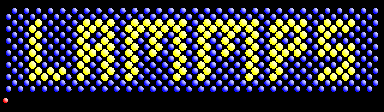
\includegraphics[width=\textwidth]{lammps-logo.png}
    \caption[lammps logo]{Image credit: https://lammps.sandia.gov/}
    \label{lammps-logo}
\end{figure}

\section{Conclusions}


%%%%%%%%%%%%%%%%%%%%%%%%%%%%%%% Ch4. Project C
\chapter{Logo of NAMD}
\graphicspath{{figures/4/}}

\section{Methods}

\begin{figure}[H]
\centering
	
\includegraphics[width=\textwidth]{namd-logo.png}
    \caption[namd logo]{Image credit: https://www.ks.uiuc.edu/Research/namd/}
    \label{namd-logo}
\end{figure}

\section{Conclusions}


%%%%%%%%%%%%%%%%%%%%%%%%%%%%%%% Ch5. Conclusion
\chapter{Conclusions}
\begin{table}[h!]
\begin{center}
\caption{Chapters of molecular dynamics package names}
\begin{tabular}{|c|c|}
\hline
Chapter  & name    \\ \hline
2        &  CHARMM \\ 
3        &  LAMMPS \\ 
4        &  NAMD   \\ \hline
\end{tabular}
\label{Tab:Tcr}
\end{center}
\end{table}

%%%%%%%%%%%%%%%%%%%%%%%%%%%%%%% Bibliography
\cleardoublepage
\addcontentsline{toc}{chapter}{Bibliography}
\bibliography{misc/bibliography}{}
\bibliographystyle{unsrt} 

\end{document}